 \vspace*{0.05cm}


\begin{center}
	
	\shadowoffset{2pt}
	\shadowrgb{0.7,0.7,0.7}
	
	\begin{blueshaded}
		\begin{center} 
			\vspace{0.25cm}
			
			{\fontfamily{phv}\fontsize{38}{57}\selectfont 
				\textbf{\shadowtext{Matemàtiques I}}
				
		
			\vspace{0.25cm}
			{\huge \textbf{1r Batxillerat de ciències}}
			}
				
			\vspace{1cm}
			\shadowoffset{1pt}
			{\Large \textbf{\shadowtext{Sèrie Pràctica}}}
			
			\vspace{0.5cm}
			
			{\Large \normalfont{\textit{3a Edició}}	}	
			\vspace{0.5cm}
		\end{center}
		
	\end{blueshaded}
	
	
	\vspace{1cm}
	
	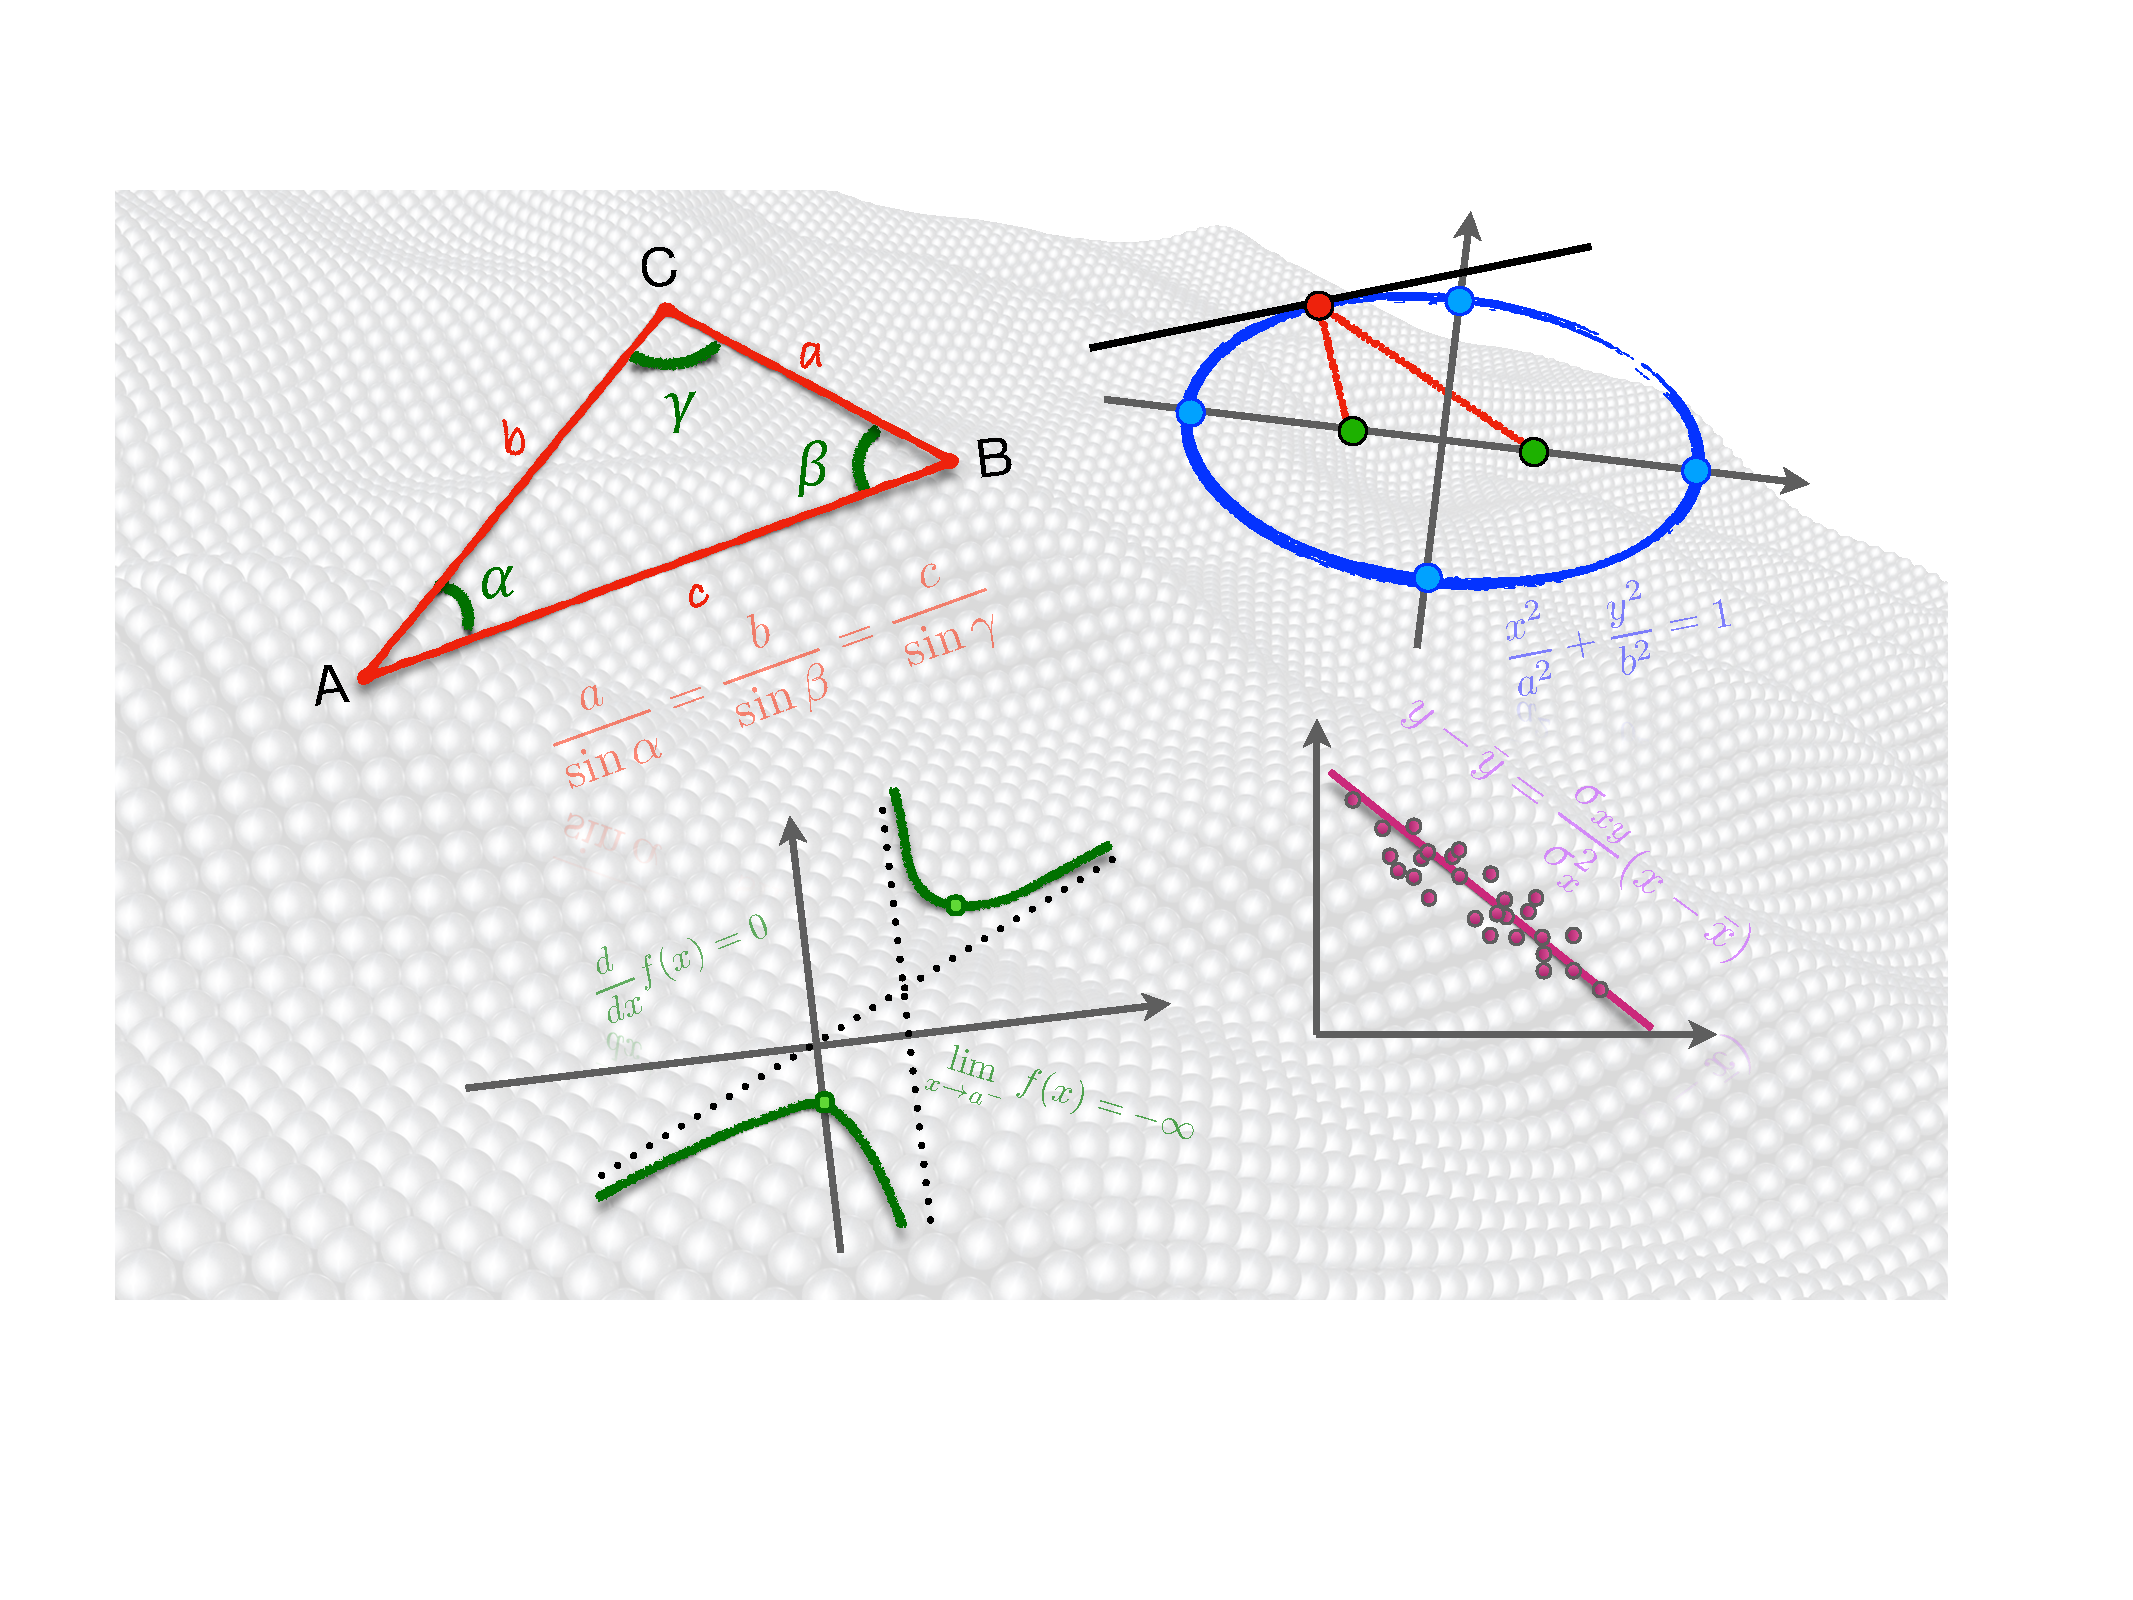
\includegraphics[width=0.9\textwidth]{img-00/portada}
	
	\vspace{1.5cm}
	
	
	\begin{minipage}{0.4\textwidth}
		\begin{center}
			\includegraphics*[width=1.2in]{img-00/ies-binissalem-logo}
			
			\small
			
			\noindent \href{www.iesbinissalem.net}{\textbf{www.iesbinissalem.net}}  
			
		\end{center}
	\end{minipage}
	\begin{minipage}{0.4\textwidth}
		\begin{flushright}
			\textbf{Josep Mulet}
			
			\textit{Departament de Matemàtiques} 
			
			IES Binissalem
		\end{flushright}
	\end{minipage} 
	
	
\end{center}

\newpage

\vspace*{12.9cm}
\begin{center}
	\begin{minipage}{0.5\textwidth}
		Aquesta és una obra derivada de ``\textit{Matematicas 1º de Bachillerato de ciencias. Ejercicios y problemas}'' de Marea Verde de matemàtiques. Per tant, està subjecta a les mateixes condicions de llicència CREATIVE COMMONS que l'obra original.
		
		\noindent \textbf{Edició \LaTeX: \quad \textregistered \,  Josep Mulet Pol}
		
		\noindent \textbf{Versió}: \quad 2018-07-31
		
		\noindent \textbf{Portada}: \quad \textit{Fractal de Julia}.
		
		
		\begin{center}
			\includegraphics*[width=8cm]{img-00/licencia}
		\end{center}
	\end{minipage}
\end{center}

%\clearemptydoublepage
%%\setcounter{page}{1}
%%\fancyfoot[C]{\roman{\thepage}}%


\newpage


\renewcommand{\thepage}{\Roman{page}}% Roman numerals for page counter
\pagestyle{myheadings}
\thispagestyle{empty}
\renewcommand{\headrulewidth}{0pt}
\renewcommand{\footrulewidth}{0pt}

\pagebreak


\dominitoc

\tableofcontents


\newpage

\heading{Currículum LOMCE}

\quad {\footnotesize Extret de \url{http://weib.caib.es/Normativa/Curriculum\_IB/batxillerat\_lomce/matematiques_batx.pdf} }

\begin{center}
	\fontsize{10.1}{13}\selectfont
	\leftmargin=0pt \itemindent=0pt 
	\begin{tabular}{|p{0.5\textwidth}|p{0.5\textwidth}|} \hline
		
		\rowcolor{lightgray} \textbf{BLOC: Nombres i Àlgebra} & \textbf{BLOC: Geometria} \\ \hline
		
		
		\begin{itemize}
			
			\item Nombres reals: necessitat del seu estudi per a la comprensió de la realitat. 
			
			\item Valor absolut. Desigualtats. Distàncies en la recta real. Intervals i entorns. 
			
			\item Aproximació i errors. Notació científica.
			
			\item Nombres complexos. Forma binomial i polar. Representacions gràfiques. Operacions elementals. Fórmula de Moivre.
			
			\item Successions numèriques: terme general, monotonia i acotació. El nombre e.
			
			\item Logaritmes decimals i neperians. Equacions logarítmiques i exponencials.
			
			\item Plantejament i resolució de problemes de la vida quotidiana mitjançant equacions i inequacions. Interpretació gràfica.
			
			\item Resolució d’equacions no algebraiques senzilles.
			Mètode de Gauss per a la resolució i interpretació de sistemes d’equacions lineals.
		\end{itemize}
		
		&
		
		\begin{itemize}
			
			\item 	Mesura d’un angle en radiants.
			
			\item Raons trigonomètriques d’un angle qualsevol. Raons trigonomètriques dels angles suma i diferència d’altres dos, doble i meitat. Fórmules de  transformacions trigonomètriques.
			
			\item Teoremes. Resolució d’equacions trigonomètriques senzilles.
			
			\item Resolució de triangles. Resolució de problemes geomètrics diversos.
			
			\item Vectors lliures en el pla. Operacions geomètriques.
			
			\item Producte escalar. Mòdul d’un vector. Angle de dos vectors.
			
			\item Bases ortogonals i ortonormals.
			
			\item Geometria mètrica plana. Equacions de la recta. Posicions relatives de rectes. Distàncies i angles. Resolució de problemes.
			
			\item Llocs geomètrics en el pla.
			
			\item Còniques. Circumferència, el·lipse, hipèrbola i paràbola. Equació i elements.
			
			
		\end{itemize}
		\\ \hline
		
		\rowcolor{lightgray}  \textbf{BLOC: Anàlisi} & \textbf{BLOC: Estadística i probabilitat}  \\ \hline
		
		\begin{itemize}
			
			\item 	Funcions reals de variable real.
			
			\item Funcions elementals: polinòmiques, racionals senzilles, valor absolut, arrel, trigonomètriques i les seves inverses, exponencials, logarítmiques i funcions definides a trossos.
			
			\item Operacions i composició de funcions. Funció inversa. Funcions d’oferta i demanda.
			
			\item Concepte de límit d’una funció en un punt i en l’infinit. Càlcul de límits. Límits laterals. Indeterminacions.
			
			\item Continuïtat d’una funció. Estudi de discontinuïtats.
			
			\item Derivada d’una funció en un punt. Interpretació geomètrica de la derivada de la funció en un punt. Recta tangent i normal.
			
			\item Funció derivada. Càlcul de funcions derivades. Regla de la cadena.
			
			\item Representació gràfica de funcions.
			
		\end{itemize}		
		&
		
		\begin{itemize}
			\item 	Estadística descriptiva bidimensional:
			Taules de contingència.
			
			\item Distribució conjunta i distribucions marginals.
			
			\item Mitjanes i desviacions típiques marginals.
			
			\item Distribucions condicionades.
			
			\item Independència de variables estadístiques.
			
			\item Estudi de la dependència de dues variables estadístiques. 
			
			\item Representació gràfica: Núvol de punts.
			
			\item Dependència lineal de dues variables estadístiques. 
			
			\item Covariància i correlació: Càlcul i interpretació del coeficient de correlació lineal.
			
			\item Regressió lineal. Estimació. Prediccions estadístiques i fiabilitat de les mateixes.
		\end{itemize}		
		\\ \hline
		
		
	\end{tabular}	
\end{center}

\cleartorightpage
 

\vspace*{2cm} 
\heading{Símbols}

\begin{center}
	\renewcommand{\arraystretch}{1.5}
	\begin{longtable}[h]{>{\raggedleft\arraybackslash}p{0.19\textwidth}|p{0.78\textwidth}}
		{\bfseries Símbol} & {\bfseries Significat} \\ \hline
		
		\simbolclau & Problema clau amb solució al final del llibre.  \\ \hline
		
		\simbolcompass & A més de la solució, proporciona orientacions per arribar a ella.  \\ \hline
		
		\simbolsearch & Problema que requereix d'investigació o recerca d'informació.  \\ \hline
		
		\ggb & Activitat adequada per realitzar amb el programa Geogebra.  \\ \hline
		
		\begin{center}
\includegraphics[width=1cm]{img-00/video-164}\par {\footnotesize Vídeo 132:}\end{center} & Explicació en vídeo dels continguts de l'apartat. El número de vídeo correspon a la numeració emprada en https://piworld.es 
		
		\\ \hline
		\hot[2] & Problema amb un cert grau de dificultat. \\ [0.25cm] \hline
		\spen & Activitat que es pot contestar en el llibre mateix. \\ [0.25cm] \hline 
		\mental & Activitat que es pot resoldre mentalment o en veu alta.
	\end{longtable}
\end{center}
\vspace{1cm} 

\heading{Recursos}

\begin{center}
	\renewcommand{\arraystretch}{1.5}
	\begin{longtable}[h]{>{\raggedleft\arraybackslash}p{0.2\textwidth}|p{0.8\textwidth}}
		\hline
		\textbf{piWorld}
		
		
\includegraphics[height=1.5cm]{img-00/piworld}
		& Plataforma d'aprenentatge. Conté explicacions en vídeo i activitats interactives. Requereix usuari i contrasenya. \newline
		\quad \href{https://piworld.es}{\href{https://piworld.es}{https://piworld.es}}
		\\ \hline
		\textbf{Geogebra} 
		
		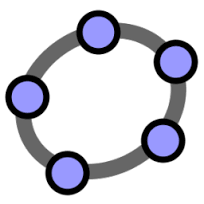
\includegraphics[height=1.5cm]{img-00/geogebra}
		& Programa lliure de geometria dinàmica en dues i tres dimensions.
		Ideal pels temes de funcions i geometria.\newline
		\quad  \href{https://www.geogebra.org/download}{\href{https://www.geogebra.org/graphing}{https://www.geogebra.org/graphing}}
		\\ \hline
		\textbf{Calculadora WIRIS}
		
		
		
\includegraphics[height=2cm]{img-00/wiris}
		& Calculadora per al càlcul simbòlic. Nova versió Web \par \quad  \href{https://calcme.com/a}{https://calcme.com/a}
		
		La versió antiga la trobareu a \par \quad  \href{http://www.wiris.net/educa.madrid.org/wiris/es/cas.html}{http://www.wiris.net/educa.madrid.org/wiris/es/cas.html}
		
		Atenció: requereix el plugin de Java i no funciona en dispositius mòbils.
		\\ \hline
		
	\end{longtable}
\end{center}
